% Very simple template for lab reports. Most common packages are already included.
\documentclass[a4paper, 11pt]{article}
\usepackage[utf8]{inputenc} % Change according your file encoding
\usepackage{graphicx}
\usepackage{url}
\usepackage{listings}
\usepackage{xcolor}

\definecolor{mygray}{rgb}{0.5,0.5,0.5}

\lstset{
    basicstyle=\footnotesize,
    language=erlang,
    frame=single,
    numbers=left,
    numberstyle=\tiny\color{mygray},
    breaklines=true,
}

%opening
\title{Routy: a small routing protocol}
\author{Antonios Kouzoupis $<$antkou$@$kth.se$>$}
\date{\today{}}

\begin{document}

\maketitle

\section{Introduction}

In this seminar we have implemented \emph{Routy}, a small yet reliable routing
protocol. The topics we have covered are how a link--state protocol works and how
to achieve consistency of a network when nodes stop working. As a consequence of
this seminar we had an even deeper look in Erlang.

Routy is a link--state protocol, which mean that every node in the network
should construct a connectivity map to other nodes. Afterwards, using
Dijkstra's algorithm, it finds the shortest path to a node and finally it builds
the routing table. Routy also uses a monitoring system in order to detect and
emend network topology changes such as failures.

\section{Main problems and solutions}

Personally, I believe that the  most difficult part of the seminar was to obtain a
solid understanding of how the protocol works. How to use the \emph{Map}, the
\emph{Sorted List} and how to combine all the different components together in
order for the router to work. So reading the seminar paper and the book was of
crucial importance to continue with the implementation.

Also, implementing Dijkstra's algorithm was not trivial. It consisted of many
operations that you had to be completely sure they worked correctly before you
proceed further. So testing was the only solution. Testing every functionality
separately and then the whole algorithm. It was very important for the algorithm
to produce the correct result since it is the heart of our routing protocol.
In Figure \ref{fig:dijkstra} is illustrated how the algorithm is implemented.
Edge cases of function are when the \emph{Sorted List} is empty or the first
element's distance is ``inf''. Then for every node that is reachable from the
node in question I update the entry in the Sorted List with new weight and
gateway. Finally I fill the routing table with the current node and gateway.

\begin{figure}[h!]
    \lstinputlisting[language=erlang]{dijkstra.erl}
    \caption{Dijkstra's algorithm}
    \label{fig:dijkstra}
\end{figure}

\emph{History} module was also of great importance since, an error in keeping
track of old messages led in infinite loop while broadcasting. Finally the
\emph{broadcast} and \emph{update} procedure was not very clear to me so I had
to run many tests and gather the output from multiple Routy instances to figure
out how routers are advertised and update their map and routing table.

\section{Evaluation}

For the evaluation procedure, I wrote a test case which started five routers,
\emph{Stockholm, Bor\aa s, Lule\aa, Ume\aa}  and \emph{Lund}. They were
connected to each other according to the topology illustrated in Figure
\ref{fig:topology}.

\begin{figure}
    \begin{center}
        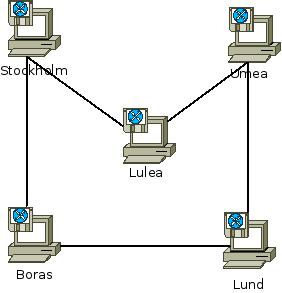
\includegraphics[scale=0.6]{network.jpeg}
        \caption{Routy network topology}
        \label{fig:topology}
    \end{center}
\end{figure}

The first scenario was to send a message from \emph{Stockholm} to \emph{Lund}.
As shown in the topology, there are two available paths, one which uses
\emph{Bor\aa s} as a gateway and another which uses \emph{Lule\aa} as a gateway
and pass from \emph{Ume\aa} to reach \emph{Lund}. Routy chooses to use the first
path since Dijkstra's algorithm indicated it as the shortest one.

The second scenario was to send a message from \emph{Stockholm} to \emph{Ume\aa}
but with \emph{Lule\aa} node down. So after I started all the nodes, broadcast and
updated the interfaces, map and routing table, I closed the \emph{Lule\aa} node
and update the map and routing table of the remaining nodes. Normally the message
would pass through \emph{Lule\aa} since it is the shortest path but because
it is down, necessarily it will pass through \emph{Bor\aa s} and \emph{Lund}.
The ``update'' function is not executed automatically, so we must explicitly
call it, otherwise our message will not be able to route. This one proves that
indeed Routy adapts to network topology changes, if a node is down it constructs
another path.

\section{Conclusions}

In this seminar we have learnt how link--state protocols, like OSPF work. We
implemented a router based on link--state and Dijkstra's algorithm. It was
really interesting to see messages routed through various nodes and construct new
paths to deal with failures. Finally, through the seminar homeworks I learn more
and more about Erlang.

\end{document}
